% LaTeX file for Chapter 02


\chapter{Data} 
Maybe it is the methods section. Here however, we give a couple hints.
Note that you can wisely use \rr{preamble}-chunks. Minimal, is likely: 

\bigskip

\hrule

\hrule

\bigskip

Defining figure options is very helpful:

 
\bigskip


\hrule

\hrule

\bigskip 

This options are best placed in the main document at the beginning. Otherwise a \verb+cache=FALSE+ as knitr option is necessary to overrule a possible  \verb+cache=TRUE+ flag. 

\bigskip 

Notice how in Figure~\ref{f02:1} everything is properly scaled.   

\begin{figure}
\begin{knitrout}
\definecolor{shadecolor}{rgb}{0.98, 0.98, 0.98}\color{fgcolor}

{\centering 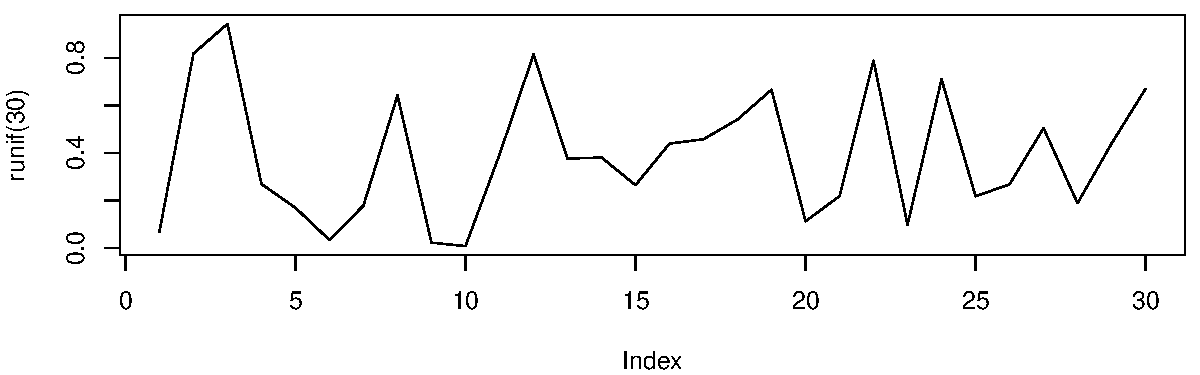
\includegraphics[width=\textwidth-3cm]{figure/ch02_figunnamed-chunk-3-1} 

}


\end{knitrout}
  \caption{Test figure to illustrate figure options used by knitr.}
  \label{f02:1}
\end{figure}


\section{Citations}

Recall the difference between \verb+\citet{}+ (e.g., \citet{Chu:Geor:99}), \verb+\citep{}+ (e.g., \citep{Chu:Geor:99}) and \verb+\citealp{}+ (e.g., \citealp{Chu:Geor:99}).
For simplicity, we include here all references in the file \verb+biblio.bib+ with the command \verb+\nocite{*}+.\nocite{*}

